\documentclass[9pt,twocolumn,twoside]{article}
\usepackage{amsmath}
\usepackage{amssymb}
\usepackage{bbm}
\usepackage{mathtools}
\usepackage{afterpage}
\usepackage{graphicx}
\usepackage{subfigure}

\usepackage{listings}
\usepackage{color}

\definecolor{dkgreen}{rgb}{0,0.6,0}
\definecolor{gray}{rgb}{0.5,0.5,0.5}
\definecolor{mauve}{rgb}{0.58,0,0.82}

\lstset{%frame=tb,
  language=Python,
  aboveskip=3mm,
  belowskip=3mm,
  showstringspaces=false,
  columns=flexible,
  basicstyle={\small\ttfamily},
  numbers=none,
  numberstyle=\tiny\color{gray},
  keywordstyle=\color{blue},
  commentstyle=\color{dkgreen},
  stringstyle=\color{mauve},
  breaklines=true,
  breakatwhitespace=true,
  tabsize=3
}


\begin{document}

\title{Lattice Gauge Theories with Discrete Gauge Groups}
\author{Hunter Swan}

\maketitle
\begin{abstract}
I describe the formulation of lattice gauge theories for a variety of discrete gauge groups, including the cyclic groups $Z_N$, the Klein 4 group $K_4$, and the quaternion group $Q$.  Using Monte Carlo methods, I map the phase diagrams for these theories in various dimensions and identify phase transitions.
\end{abstract}

\section{Introduction}
Quantum field theory is \textit{hard}.  The playing field for quantum field theory (QFT) is a massively infinite dimensional Hilbert space, and the players themselves are operator valued functions of spacetime coordinates with infinitely many quantum degrees of freedom.  The dynamics are represented by functional integrals---infinite dimensional integrals over the space of fields---which by their nature are impossible to compute in any concrete way (e.g. on a computer via some sort of quadrature), and usually don't have the decency to converge anyway.  As if to add insult to injury, even in those cases where one can evaluate a quantity in QFT, it often turns out to be $\infty$ (perhaps not a surprise, given the number of infinities encountered already in this paragraph).  The situation is so desperate, mathematicians have put up a million dollar bounty for the first person to tame QFT.

Despite its lack of aesthetic appeal, QFT is apparently \textit{right}, insofar as we can tell.  That is to say, QFT still manages to make predictions, and those predictions are in exquisite agreement with reality (for example, the theory of quantum electrodynamics, QED, has been tested to 15 decimal places with no deviations so far).  So regardless of our possible prejudices against the mathematical or computational character of QFT, we pretty much have to live with it.  The burden therefore seems to be on us, the examiners, to reconcile ourselves to QFT, rather than holding out for QFT to reconcile itself to our ideologies.  

Enter \textbf{lattice quantum field theory} (LQFT).  This is the same as regular QFT (which we shall refer to as continuum QFT or CQFT for the purposes of differentiating the two), but with spacetime discretized on a lattice.  This seems innocent enough, and in fact it \textit{is} far more innocent than its reprobate cousin CQFT: LQFT is perfectly well-defined mathematically, and even numerically tractable.  What makes LQFT even more attractive is that, by taking appropriate continuum limits, it can provide answers to questions of CQFT!

So the first reason we should care about LQFT is that it provides a palatable and productive way to approach continuum QFT.  However, even apart from continuum limits, LQFT has interesting structure in its own right.  Some lattice quantum field theories turn out to be exactly equivalent to systems arising from statistical mechanics, and as such they display the same sorts of phase transitions and critical behavior characteristic of the latter systems.  LQFT thus provides a new perspective on statistical mechanics, helping elucidate the structure of systems with many degrees of freedom.  This is roughly the thrust of the present paper.  My main goal is to look at a variety of lattice gauge theories (particular kinds of LQFT, to be defined below) and examine how the phase structure of the theory depends on its intrinsic properties (namely, its gauge group, action, and the dimension of the ambient lattice).  (This has been shown to be an interesting paradigm before \cite{Creutz,DAdda,Rebbi,Grosse}, and I'll revisit some of this work below.)

\section{Definitions and QFT background}
Normally, one thinks of quantum field theory as residing in Minkowski space, i.e. $\mathbb{R}^4$ with metric $ds^2 = -dt^2 + dx^2 + dy^2 + dz^2$.  Physicists like to say that this metric puts time and space ``on equal footing''.  The argument goes something like this: ``Blah blah blah blah special relativity blah blah blah.''  Of course this argument is total hogwash: Any preschooler can tell you that the time coordinate in this metric gets a minus sign, while the space coordinates have plus signs.  There is a cure, though!  If we set $\tau := \pm i t$, then we can rewrite the metric as $ds^2 = d\tau^2 + dx^2 + dy^2 + dz^2$.  Now the ``imaginary time'' coordinate $\tau$ really is on equal footing with the spatial coordinates.  What we've done essentially is to embed $\mathbb{R}^4$ into $\mathbb{C}\times \mathbb{R}^3$ and then restrict to the imaginary axis of $\mathbb{C}$.  Geometrically we haven't done anything fancy.  However, once we start considering functions of $\mathbb{R}^4$ (fields), in order for the corresponding rotation of the functions to be unambiguous we will need to ensure that they all are analytic in time, so that we can uniquely extend them from the reals to the complex plane.  Fortunately, physicists are confident that this can be done in all the cases we care about.  The proof goes as follows: If we were to find a function which was non-analytic so that we could not rotate it in this way, then by definition, we no longer care about it.  QED

So assume that we can do this rotation in the complex $t$-plane (this is called a Wick rotation).  After this section we will always work in this Wick rotated space.  The rationale for doing this is partly, as mentioned above, to symmetrize the roles of time and space coordinates, but another reason stems from the effect this has on dynamics of a quantum field theory.  Loosely speaking, putting an $i$ in a function argument turns oscillatory behavior into exponentially growing/decaying behavior and vice versa (as is the case for e.g. $\sin(\cdot)$, $\cos(\cdot)$, and $\exp(\cdot)$).  Oscillating functions are bad for integrals: They take forever to converge (if they converge at all), and the eventual value of the integral depends on lots of cancellation of regions with different phase.  By contrast, exponentially decaying functions exhibit no such pathologies---they are a complete joy to integrate.  Dynamics of quantum field theory in Minkowski space is described by an oscillatory integral.  After Wick rotation, this oscillatory integral becomes a much better behaved integral with an exponentially damped integrand.  This makes it far preferable for numerical work (not to mention rigorous mathematical work, where the Wick rotated integral has a fully satisfactory definition, whereas the oscillatory integral has thus far only been established precisely in a few cases).  We will see how this comes about explicitly in a little bit, but first we lay down some terminology:

%About the only function we will ever need to actually perform this rotation on is the action.  We'll do that in just a bit, after we lay down some definitions:

\begin{itemize}
\item A \textit{continuum field} is a function on $\mathbb{R}^n$.  Continuum fields are typically either scalar or vector valued (classical fields) or operator valued (quantum fields).
\item An \textit{action} is a real-valued function of one or more continuum fields.
\item A \textit{continuum field theory} is a collection of continuum fields over the same space, together with an action on those fields and an additional set of prioritized functions of the fields called \textit{observables}.
\item A \textit{lattice}, for our purposes, is a graph with vertices $\mathbb{Z}_{m_1}\times\mathbb{Z}_{m_2}\times \cdots \times \mathbb{Z}_{m_n}$ and edges connecting two vertices if and only if those vertices' coordinates differ by exactly one unit (mod $m_j$) in exactly one direction $j$.  We will speak of an edge being ``in direction $j$'' if the vertices it connects are adjacent in that direction.  The (mod $m_j$) means we're making everything periodic from the get-go.  The lattice has associated with it a \textit{lattice spacing} $a_0$, which describes the distance between lattice points when embedded into $\mathbb{R}^n$.  We'll only need one lattice at a time in this paper, which we will call $L$, and since we won't be taking any continuum limits we will generally forget about the lattice spacing $a_0$.  We will use the following notation for talking about lattices: $V(L)$ will denote the vertices of $L$; $E(L)$ will denote the edges of $L$; and for any edge $e\in E(L)$ in direction $j$ with vertices $v,w\in V(L)$, if $v_j-w_j\equiv 1$ (mod $m_j$) we set $e_- = w$ and $e_+ = v$, i.e. $e_-$ is the ``lower'' vertex of $e$ and $e_+$ is the ``upper'' vertex.  (This definition of $e_-$ and $e_+$ is ambiguous when $m_j\leq 2$, so we will always require that $L$ have more than 2 points in all directions.)
\item A \textit{lattice field} is a function of a lattice's edges or vertices.  Most of the fields we will be interested in for this paper will take values in a group (the local symmetry group of the theory).  We use the term \textit{field} to refer to either a lattice field or continuum field, depending on context.
\item \textit{Lattice action} and \textit{lattice field theory} are defined analogously to the continuum case. 
\item A \textit{gauge group} $\mathcal{G}$ is a set of fields $T$ taking values in a group $G$, called the local symmetry group.  We require that $\mathcal{G}$ be closed under pointwise multiplication of such fields $T$.  As the name suggests, $\mathcal{G}$ is itself a group, with the group operation given by pointwise multiplication of fields.  In the continuum case, all the fields $T\in\mathcal{G}$ should be smooth.
\item A \textit{gauge theory} (lattice or continuum) is a field theory together with a gauge group $\mathcal{G}$ and a group action of $\mathcal{G}$ on the fields of the field theory, such that the action and all observables are invariant under the group action.  The group action by any particular element $T \in G$ is called a \textit{gauge transformation}.  Sometimes we also refer to $T$ itself as a gauge transformation.
\end{itemize}

Lattice gauge theories are the objects of interest in this paper.  I have so far provided no motivation for why gauge theories are more interesting than any other field theory.  I think the best explanation is simply that they exist: quantum electrodynamics, the electroweak interaction, and quantum chromodynamics are all gauge field theories.  I don't know a principled reason \textit{why} these theories should be gauge theories, but regardless, they are, and ergo we study gauge theories.

Many of the commonly studied lattice gauge theories are inherited from the continuum field theories of the standard model (especially quantum chromodynamics).  It turns out there is a reasonably algorithmic way to turn continuum field theories into lattice theories, as follows:
\begin{enumerate}
\item Wick rotate the action (and any relevant observables). 
\item Discretize space onto a lattice, thereby making all continuum fields lattice fields.
\item Choose a lattice action which reduces to the Wick rotated continuum action as the lattice spacing vanishes.
\end{enumerate}

This prescription is not totally algorithmic, because (for one thing) there can be many lattice actions that reduce to the same continuum action.  Moreover, there are lots of potentially interesting lattice field theories which cannot be obtained in this manner---an issue we will take up in the next section.

As an example of how this works in practice, consider a free scalar field in Minkowski space, $\phi:\mathbb{R}^n\rightarrow \mathbb{R}$, with action defined as 
\[S[\phi] := \int d^nx \frac{1}{2}(\partial_{\mu}\phi) (\partial^{\mu}\phi) - \frac{1}{2}m^2\phi^2.\]
After Wick rotating $t$ to $-it$, the $(\partial_0\phi)^2$ term picks up a $-1$ and the measure $dt$ picks up a $-i$, so the action becomes
\[i \int d^nx \frac{1}{2}(\partial_0\phi)^2 + \frac{1}{2}(\nabla\phi)^2 + \frac{1}{2}m^2\phi^2 =: i S_E[\phi].\]
$S_E[\phi]$ is called the Euclidean action.  It can be discretized onto a lattice in an obvious way:
\[ S_E[\phi] \rightarrow a_0^n \sum_{x\in V(L)} \left( \frac{1}{2}m^2\phi(x)^2 + \frac{1}{2} \sum_{\mu=0}^n (\nabla_{\mu} \phi(x))^2 \right),\]
where we have introduced the notation $\nabla_{\mu} \phi(x) := (\phi(x+\hat{e}_{\mu}) - \phi(x))/a_0$ (with $\hat{e}_{\mu}$ the unit vector in direction $\mu$ and $a_0$ the lattice spacing) for the discrete derivative.  This discretization is not at all unique (Homework Exercise 1: find another discretization), but coarse physics like phase structure should not depend on the choice of discretization anyway.  

In Minkowski spacetime, the entities we try to compute from a quantum field theory are expressed in terms of functional integrals over all field configurations $\phi$, weighted by $\exp(i S[\phi])$.  E.g. the expectation of an operator $A(x,y,...)$ is given by
\[\left<A(x,y,...)\right> = \frac{\int \mathcal{D}\phi \: A(x_1,x_2,...) \exp(i S[\phi])}{\int \mathcal{D}\phi \: \exp(i S[\phi])}, \]
where $\int \mathcal{D}\phi$ means a functional integral over all configurations of $\phi$.  (This integral is tricky to define precisely for continuum fields, but when we discretize onto a lattice shortly it will become very well-defined.)  These are the oscillatory integrals alluded to earlier, with the oscillations coming from the $\exp(i S[\phi])$ factor.  After Wick rotation this oscillatory term becomes a decaying exponential:
\[\frac{\int \mathcal{D}\phi \: A(x,y,...) \exp(-S_E[\phi])}{\int \mathcal{D}\phi \: \exp(-S_E[\phi])}.\]
Note that $x_0,y_0,...$ are (implicitly) rotated by $-i$ in this formula.  These Wick rotated integrals are ostensibly nicer, because of the exponential damping term.  They're still awfully big though, because we're integrating over an infinite dimensional space of fields.  Let's put everything on a lattice to salve our conscience:
\[ \left<A(x,y,...)\right> \rightarrow \frac{\prod_{z\in V(L)}\int d\phi(z) \: \phi(x)\phi(y) \exp(-S_E[\phi])}{\prod_{z\in V(L)}\int d\phi(z) \: \exp(-S_E[\phi])}\]
All we've done is replace $\int \mathcal{D}\phi$ with $\prod_{z\in V(L)}\int d\phi(z)$.  That is, integrating over all field configurations is now just integrating over the values of $\phi$ at each lattice site.  There are a finite number of lattice sites, so this is now a finite dimensional integral, which is something you can think of doing on a computer.  However, it's still still awefully big---the number of integrations is the number of lattice points, which can be thousands to millions or more for reasonably sized lattices.  Evaluating this efficiently is typically accomplished via Monte Carlo methods, which we will describe below.  For now, though, we finish the job at hand by identifying what we will want to compute when we get there.  The denominator of the above expression
\[Z := \prod_{z\in V(L)}\int d\phi(z) \: \exp(-S_E[\phi])\]
is recognized as essentially a partition function with Hamiltonian function $\mathcal{H}[\phi] := S_E[\phi]$ and inverse temperature $\beta=1$.  This looks worth computing.  It would probably be cooler if we could change the temperature $\beta$, so that it wasn't fixed at 1.  So redefine
\[Z(\beta) := \prod_{z\in V(L)}\int d\phi(z) \: \exp(-\beta S_E[\phi]).\]
The free energy is then defined in the usual way:
\begin{align*}
F(\beta)& := -\frac{d \log(Z)}{d\beta}\\
& = \frac{1}{Z}  \prod_{z\in V(L)}\int d\phi(z) \: S_E[\phi] \exp(-\beta S_E[\phi]).
\end{align*}
That is, the free energy is the expectation value of the action.  Free energy in this form is extrinsic, so to get a statistic that doesn't grow with lattice size we look at the free energy per site $f(\beta):=F(\beta)/N$, where $N$ is the number of lattice sites.  This is one of the basic quantities of interest to us in this paper.  The other is the heat capacity 
\begin{eqnarray*}
c(\beta)& := & \frac{-1}{N}\frac{df}{d\beta}\\
& = & \frac{1}{N^2}\frac{1}{Z}  \prod_{z\in V(L)}\int d\phi(z) \: S_E[\phi]^2 \exp(-\beta S_E[\phi]) \\
& & -\frac{1}{N^2}\frac{1}{Z^2} \left( \prod_{z\in V(L)}\int d\phi(z) \: S_E[\phi] \exp(-\beta S_E[\phi])\right)^2 \\
& = & \frac{1}{N^2}\left(\left<S_E^2\right> - \left<S_E\right>^2\right)
\end{eqnarray*}

The generalization to multiple fields, defined on either vertices or edges of $L$, is straightforward: Just replace the integration measure $\prod_{x \in V(L)}  d\phi(x)$ by the product measure over all degrees of freedom, i.e. the field values at all edges or vertices.  If $\phi$ maps into a finite set, the integral becomes a sum.  For intrinsic quantities, divide by the total number of degrees of freedom (instead of by $N$ as above).

\section{Lattice gauge theories}
We now introduce concretely the stars of our show: lattice gauge theories (LGTs).  The form of the LGTs we consider has its genesis in discretizations of the Yang-Mills continuum field theory.  I won't go through the discretization here---I'll just state the result.  (Homework Exercise 2: Discretize the standard model.)

An LGT is specified by four things:
\begin{enumerate}
\item The lattice $L$.
\item Some fields $\{u_i\}$ on the lattice.
\item A gauge group $\mathcal{G}$ (with local symmetry group $G$) along with a group action on the fields $\{u_i\}$.
\item An action $S[\{u_i\}]$ and some observables $\{A[\{u_i\}]\}$, which should be invariant under gauge transformations.
\end{enumerate}

Our LGTs will consist of a single field $u(e)$ which lives on edges $E(L)$ of the lattice and takes values in the local symmetry group $G$.  The gauge group is the set of all $G$-valued fields $T$ on the \textit{vertices} $V(L)$.  The group action of a gauge transformation $T\in\mathcal{G}$ on $u$ is given by 
\begin{equation}
(T\cdot u)(e) = T(e_-) u(e) T(e_+)^{-1}
\label{gaugeAction}
\end{equation}
for any edge $e\in E(L)$.  This describes items (1)-(3) of the above list.  To describe the form of the last item---the action and observables---we must foray into some more detailed group theoretic considerations.  This is important enough it deserves its own subsection:

\subsection{Gauge invariance and group theory}
The action and observables of our LGTs must be functions of $u$ which are invariant under gauge transformations.  Now, looking at the form (\ref{gaugeAction}) of the gauge group action given above, we see that gauge transformations can make the value of $u$ at a given edge $e$ be anything whatsoever---for example, taking $T(e_+)=u(e)$ makes the transformed value $(T\cdot u)(e) = T(e_-) u(e) u(e)^{-1} = T(e_-)$, which is totally arbitrary.  So no function of $u$ at a single point in the lattice will be gauge invariant (except boring constant functions).  

To see what kinds of functions of $u$ \textit{are} gauge invariant, consider a product of the form $u(e^1)u(e^2)\cdots u(e^k)$, where the $e^j$ are edges satisfying $e_+^j=e_-^{j+1}$ for all $j\in\{1,2,...,k-1\}$.  That is, the edges form a \textit{path} of length k.  Under a gauge transformation $T$, we have 
\begin{multline*}
u(e^1)u(e^2)\cdots u(e^k) \rightarrow  \\
T(e_-^1)u(e^1)T(e_+^1)^{-1} T(e_-^2)u(e^2)T(e_+^2)^{-1} \cdots T(e_-^k)u(e^k)T(e_+^k)^{-1} \\ 
=  T(e_-^1)u(e^1)u(e^2)\cdots u(e^k)T(e_+^k). 
\end{multline*}
The factors of $T(\cdot)$ in the middle of the transformed product all cancel, leaving just the factors for the endpoints of the path.  So such a product along a path is \textit{almost} gauge invariant!  However, note the above requirement $e_+^j=e_-^{j+1}$ restricts us to paths that only move from lower vertices to upper vertices (what we will call the ``forward'' direction) of each edge along the way.  In general we would like to be able to traverse an edge in either direction, forward or backward.  Such a general path we will write as $(\pm_1 e^1, \pm_2 e^2, \dots , \pm_k e^k)$, where a $+e^j$ means edge $e^j$ is traversed forward and a $-e^j$ means it is traversed backward (the subscripts on the $\pm$ signs are just labels to differentiate them).  For this to give a well-defined path we must have $e^j_{\pm_j} = e^{j+1}_{\mp_{j+1}}$ (where $\mp_j$ indicates the sign opposite to $\pm_j$).  To make an \textit{almost} gauge invariant quantity out of the values $u(e^j)$ along this path, we construct the product 
\[P(\pm_1 e^1, \pm_2 e^2, \dots , \pm_k e^k) := u(e^1)^{\pm_1 1} u(e^2)^{\pm_2 1} \cdots u(e^k)^{\pm_k 1}.\]
For example 
\[P(-e^1,+e^2,\dots,+e^k) = u(e^1)^{-1} u(e^2)\cdots u(e^k).\]
I claim that this product is almost gauge invariant, in the same sense as before:
\begin{multline*}
P(\pm_1 e^1,\pm_2 e^2,\dots,\pm_k e^k) \rightarrow \\
\left(T(e_-^1)u(e^1)T(e_+^1)^{-1}\right)^{\pm_1} \cdots \left(T(e_-^k)u(e^k)T(e_+^k)^{-1}\right)^{\pm_k} \\
= T(e_{\mp_1}^1) u(e^1) u(e^2) \cdots u(e^k) T(e_{\pm_k}^k)^{-1} \\
= T(e_{\mp_1}^1) P(\pm_1 e^1,\pm_2 e^2,\dots,\pm_k e^k) T(e_{\pm_k}^k)^{-1}
\end{multline*}
The requirement $e^j_{\pm_j} = e^{j+1}_{\mp_{j+1}}$ produces the desired cancellation of most of the factors $T(\cdot)$.  

Now there's some bad news: For a path $(\pm_1 e^1, \dots , \pm_k e^k)$ which starts and ends at different points, the value $P(\pm_1 e^1, \dots , \pm_k e^k)$ can still be made to have arbitrary value by gauge transforming, using the same argument as for the case of a single edge.  However, if the path starts and ends at the same point---i.e. it is a loop---then $e_{\mp_1}^1 = e_{\pm_k}^k =: v_0$, and the product transforms as 
\begin{multline*}
P(\pm_1 e^1,\dots,\pm_k e^k) \rightarrow \\
= T(v_0) P(\pm_1 e^1,\dots,\pm_k e^k) T(v_0)^{-1}
\end{multline*}

This transformation is precisely \textit{conjugation by $T(v_0)$}.  This conjugation operation does not allow the value of the product to be completely arbitrary.  For example, if the group $G$ is Abelian, then $T(v_0) P(\pm_1 e^1,\dots,\pm_k e^k) T(v_0)^{-1} = P(\pm_1 e^1,\dots,\pm_k e^k)$, so the product is gauge invariant!  Even if $G$ is not Abelian, the values that the product can be transformed to are restricted to lie in the same \textit{conjugacy class}.  (The conjugacy class of an element $g\in G$ is the set $Cl(g):=\{hgh^{-1} : h\in G\}$.  It's not hard to show that these classes define an equivalence relation on $G$ and are invariant under conjugation by any element $h\in G$.  So in particular, conjugation by $T(v_0)$ does not change the conjugacy class of $ P(\pm_1 e^1,\dots,\pm_k e^k)$.)  This means the conjugacy class $Cl( P(\pm_1 e^1,\dots,\pm_k e^k) )$ is gauge invariant. 

In addition to gauge invariance, the conjugacy class $Cl( P(\pm_1 e^1,\dots,\pm_k e^k) )$ also has the nice property of being invariant under cyclic permutations of the edges,
\begin{eqnarray*}
& & Cl\left( P(\pm_2 e^2,\dots,\pm_k e^k,\pm_1 e^1)\right) \\
& = & Cl\left(  u(e^2)^{\pm_2 1} \cdots u(e^k)^{\pm_k 1} u(e^1)^{\pm_1 1} \right) \\
& = & u(e^1)^{\pm_1 1} Cl\left( u(e^2)^{\pm_2 1} \cdots u(e^1)^{\pm_1 1} \right)  u(e^1)^{\mp_1 1} \\
& = & Cl\left(  u(e^1)^{\pm_1 1} u(e^2)^{\pm_2 1} \cdots u(e^k)^{\pm_k 1} \right) \\
& = & Cl\left( P(\pm_1 e^1,\pm_2 e^2,\dots,\pm_k e^k)\right). \\
\end{eqnarray*}
So the conjugacy class is a property of the loop itself, independent of the order in which we parametrize it.  We will thus sometimes abbreviate our notation and write $Cl(u,l)$ for the conjugacy class of the above product of $u$ around the edges of a loop $l$.  

We are now in a position to describe the general form of a gauge invariant action (or observable) on fields $u$:  For any loop $l$, a \textit{loop operator} $A_l[u]$ is any function of $Cl(u,l)$.  Since $Cl(u,l)$ is gauge invariant, so is $A_l[u]$.  Furthermore, any composite function of multiple loop operators---e.g. the sum $A_{l_1}[u] + A_{l_2}[u]$ of two different loop operators---is also gauge invariant.  Such composite functions are what we will take as our operators and action.  It's that simple!

Having spelled out the general form of a gauge invariant action, we will now immediately specialize to the particular form of action which is most important.  (By ``most important'' I mean ``what everybody else is using''.)  The action $S[u]$ we will consider from here on is given by a sum over all \textit{plaquettes} $P$ (that is, square loops with one edge per side) of some real-valued function $s(Cl[u,P])$, where $s$ is an arbitrary real-valued function which I will call the \textit{plaquette action}.  The arbitrariness of $s$ means that this form of action is still quite broad.  When we start doing computations, we will explore different possibilities for the plaquette action.  However, it is also nice to have a certain standard form of plaquette action that we can use as a baseline, allowing us to make comparisons between different local symmetry groups $G$, for example.  To this end, define a baseline plaquette action $\delta(\cdot)$ by 

\begin{equation}
\delta(x) = 
\begin{cases}
0 & x = Cl(\mathbbm{1}_G) \\
1 & x \neq Cl(\mathbbm{1}_G) \\
\end{cases}
\end{equation}
where $\mathbbm{1}_G$ is the identity element of $G$.  Since all groups have an identity element, this baseline action always makes sense.  (Actually, the situation is even rosier than that: For any group $G$, the conjugacy class of the identity element consists of just the identity element itself.  In symbols, $Cl(\mathbbm{1}_G) = \{h\mathbbm{1}_G h^{-1} : h\in G\} = \{\mathbbm{1}_G\}$.  So this baseline action is very similar from one group to another.)  Physically, the interpretation of this action is that a plaquette is in its ``ground state'' when the product of the edges is the identity element, and any departure from this costs a uniform amount of energy.

To be totally concrete, the LGT action arising from this baseline plaquette action is 
\[S[u] = \sum_P \delta\left(Cl(u,P)\right),\]
where the sum is over all plaquettes.  With this action in hand we now have a fully specified lattice gauge theory, for any given gauge group $G$.  

Let me dwell on this last remark a bit: We have just constructed a lattice gauge theory for totally arbitrary local symmetry group $G$.  In particular, $G$ may be discrete.  This is in stark contrast to continuum gauge theories, where local symmetry groups are always continuous.  This is because of the requirement that gauge transformations be smooth, and thus continuous.  Any continuous function of a connected space (such as $\mathbb{R}^n$) into a discrete space must be constant, so a gauge transformation coming from a discrete local symmetry group must be constant, i.e. a global symmetry.  Gauge transformations on a lattice do not have this restriction, because a lattices are not connected.  This means we have lots of gauge theories on lattices that have no analog in the continuum.  These are the sorts of LGTs we will explore below. 

\subsection{A note on gauge invariance and partition functions}
A technical point I have hitherto not mentioned is that, in gauge theories, the philosophy is to consider all field configurations which can be mapped into each other by a gauge transformation as \textit{the same state}.  This means that, technically, the states of our systems are equivalence classes of fields $u$ modulo the gauge group action.  Thus, the principled way of writing a quantity like the partition function is to sum, not over all fields $u$, but rather over all equivalence classes of fields, or equivalently over one field for each equivalence class.  There are ways to implement this (gauge fixing), but it turns out not to make any difference for the quantities we're interested in.  The reason is that, since all observables take the same values on any two gauge-equivalent fields, summing over all fields is the same as summing over all equivalence classes of fields $|\mathcal{G}|$ times ($|\mathcal{G}|$ being the gauge group size, or more generally the gauge group measure for continuous groups).  Since the observables we're interested in have two sums over states, one in the numerator and one in the denominator, this overall constant cancels, and we get the same result from summing over fields or summing over equivalence classes.  When we do simulations, we will sum over all fields, because this turns out to be easier to implement.

\section{Monte Carlo techniques}
Typical lattice gauge theory simulations are done on lattices having $\sim 10^4$ vertices, and comparable numbers of edges (to be precise, for a rectangular lattice the number of edges equals the number of vertices times the dimension of the lattice).  For the smallest local symmetry group imaginable, $\mathbb{Z}_2$, this means the number of field configurations to sum over is $\sim 2^{10^4}\sim 10^{3010}\sim$ googol$^{30}$.  This is a bigger sum than most people can do in their head, even with a good night's sleep.  This is a bigger sum than most people can do on their laptop, even with Python.  This is a bigger sum than most people can do on a supercomputer, even with a very generous grant.  

So we have to come up with something else.  The something else is Monte Carlo simulation.  The basic idea is to sum not over all states, but rather over a representative subset.  In particular, recall that all the sums we want to do contain a Boltzmann weight $\exp(-\beta S[u])$.  For states where $S[u]$ is large compared to $1/\beta$, the Boltzmann weight is tiny, and that state doesn't contribute much to the sum.  So we don't need to pay as much attention to states with large action.  Conversely, we need to care a lot about states with small action.  The key idea of Monte Carlo simulation is to pick more of the states with small action than large action.  This is done by selecting states probabilistically, with the probability of selecting a given state proportional to its Boltzmann weight $\exp(-\beta S[u])$.  It can be proven that as we pick more and more states in this way, the sum over these states (which I'll call the ``Monte Carlo sum'') converges in a nice way to the sum over \textit{all} states, which is precisely what we want.  Crucially, the Monte Carlo sum involves a manageable number of states, so this technique is one we can deploy usefully on a computer. 

More concretely, the algorithm (that I use) for doing a Monte Carlo simulation of a lattice gauge theory is as follows:
\begin{enumerate}
\item Starting from any given field configuration $u$ and some edge $e$, randomly select a group element $g\in G$ and evaluate the action $S[\cdot]$ twice: once on the original field configuration $u$ and again on the field configuration with $u(e)$ set to the new value $g$.  Call the first action $S_1$ and the second $S_2$.
\item If $S_2\leq S_1$, set the value of $u(e)$ to $g$.  Otherwise, uniformly choose a random real number $r\in [0,1)$.  If $r<\exp\left(-\beta (S_2-S_1)\right)$, then again set the value of $u(e)$ to $g$.  Otherwise leave the value $u(e)$ where it's at.
\item Repeat steps (1)-(2) (collectively known as the \textit{Metropolis algorithm}) for many edges $e$, either by going sequentially through each edge of the lattice, or else by just randomly picking many edges.  This is called a \textit{sweep} of the lattice.
\item Do many such sweeps of the lattice.  Occasionally, record the values of\ any observables $A[u]$ you care about.  We'll call the recorded values $A_1,A_2,...,A_\#$.
\end{enumerate}

The only step of this algorithm that isn't fairly self-explanatory is (2), called the \textit{acceptance rule}.  The particular form of this acceptance rule is chosen so that the new field configurations $u$ produced by this algorithm occur with a probability proportional to their Boltzmann weight $\exp(-\beta S[u])$.

The important theorem (which we will not prove) is that as $\#\rightarrow \infty$, the average value $\frac{1}{\#} \sum_i A_i$ (what I call the Monte Carlo sum) converges to the actual expectation value
\[ \left<A\right> = \frac{1}{Z(\beta)}\prod_e \int du(e) A[u] \exp\left(-\beta S[u]\right).\]

(Note that the Monte Carlo sum $\frac{1}{\#} \sum_i A_i$ doesn't contain the exponential weighting factor.  This is because the Metropolis algorithm picks states in proportion to their Boltzmann weight, so the set of values $\{A_i\}$ already has this weighting ``built in''.)  The value of the Monte Carlo sum we get from any particular simulation is randomly distributed around the true expectation value $\left<A\right>$, with a standard deviation $\sigma_{MC}$ of the form 
\begin{equation}
\sigma_{MC} \sim \sqrt{\frac{\left<A^2\right>-\left<A\right>^2}{\#-1}} = \frac{\sigma_A}{\sqrt{\#-1}},
\end{equation}
where $\sigma_A$ is the true standard deviation of $A$ over all field configurations $u$.  The $1/\sqrt{\#-1}$ in this formula comes from the Law of Large Numbers, and tells you how big you need to make $\#$ to get a desired level of accuracy:  $\sigma_A$ is typically of order $\left<A\right>$ or smaller, so to get 1\% accuracy we need $\# \approx 10^4$, to get 10\% accuracy, we need $\#\approx 100$, etc.  Crucially, this is \textit{independent of the dimension of the sum!}  (That is, independent of the number of edges in the lattice.)

One technical issue in the above Monte Carlo method is that, since new states are generated as modifications of previous states, there may be correlations from one state to the next.  This is why, in the final step, I said to record values of the operators \textit{occasionally}, rather than after every change of state.  The number of sweeps between recording values of the operators should be longer than the ``relaxation time'' of the system, i.e. the number of sweeps needed to decorrelate the new state from an old one.  Usually this is not a big deal---a sweep or two will typically suffice to decorrelate the system.  

\subsection{Metrics for Monte Carlo}
As mentioned previously, the main quantity of interest to us here is the free energy per degree of freedom (that is, per plaquette),
\[f(\beta) = \left<\frac{S}{N}\right> = \frac{1}{N}\frac{1}{Z} \prod_{e\in E(L)} \int du(e) S[u] \exp(-\beta S[u]). \]
We'll also look at the heat capacity 
\[c(\beta) = \left<\frac{S^2}{N^2}\right> - \left< \frac{S}{N}\right>^2,\]
but it's harder to get good statistics for heat capacity than it is for free energy (variance converges slower than mean).  

So our general program is to set the inverse temperature $\beta$ to various values and evaluate these observables.  What we're looking for is primarily phase transitions, which can be signaled by abrupt changes in the free energy or spikes in the heat capacity at the critical temperature.  Another useful way to find phase transitions is to sweep the system from low temperature to high temperature and back (or from high to low and back).  It often happens that near a phase transition (especially a first order phase transition) there are multiple distinct metastable states of the system, some corresponding to the low temperature phase and others to the high temperature phase.  When the system's temperature is tuned to criticality, it tends to track different metastable states depending on whether it was brought from low or high temperature, resulting in \textit{hysteresis} when the temperature is swept back and forth \cite{Creutz}.  These hysteresis cycles are in some sense a failure to equilibrate properly near the phase transition.  However, this is a ``bug that's a feature'', since it provides a good way of \textit{finding} phase transitions.  This technique will be one of our main tools.  

Once we've tentatively identified a phase transition temperature, we can zero in on it by the following protocol:  Choose an initial field $u$ such that on one half of the lattice $u$ is uniformly the group identity, and on the other half it is completely (uniformly) random.  The two halves of the lattice roughly correspond to low and high temperature states, respectively, so the overall field configuration can be considered as having a phase boundary.  If we then set the temperature of the field below the critical temperature, the low temperature phase will overtake the high temperature phase, and the energy of the system will decrease as we equilibrate the field (sweep the lattice).  Similarly, above the critical temperature the energy will increase with equilibration.  Note that this is essentially just a fancy way of defeating the metastability characteristic of the region around the phase transition.  The relative merit of this method (which I'll call the ``phase boundary method'') vs. the hysteresis method is only apparent from trying them both and seeing how they work.  It turns out that the phase boundary method gives a more precise measure of transition temperatures than the hysteresis method.  We'll use both.  

There are various other useful ways to examine the state of a Monte Carlo simulation, too: You can look at the action around some particular loop; you can count the occurrences of a particular group element; or you can just look pictures of the lattice.  These can all be useful from time to time.  

\section{Gauge.py}
I've implemented a general-purpose LGT simulator in Python, dubbed gauge.py.  The basic structure of the code is encapsulated in three classes: 
\begin{itemize}
\item A Lattice class that contains a few arrays representing the lattice.  The most important array is for the edges of the lattice, since that's where the gauge field $u$ lives, and this is where the actual values $u(e)$ for each edge $e$ are stored.  This array has shape $(m_1,m_2,...,m_n,n)$, where $n$ is the number of dimensions of the lattice and $m_j$ is the lattice size in dimension $j$.  As implemented, $n$ is arbitrary, but there's not much point in making $n<2$, and you're pushing your luck to try anything bigger than about $n=4$, unless you have a lot of spare petaflops lying around.  (I did try $n=5$ with a 5 by 5 by 5 by 5 by 5 lattice.  It worked.  High five!) 

In the present code, I also have arrays for addressing plaquettes, either from the ``lower left vertex'' and two directions, or from an edge and a second direction.  These provide a slightly faster way of finding the plaquettes, at the expense of additional memory overhead. 
\item A Group class allows the specification of arbitrary groups by their multiplication table.  Group elements are labeled by integers $0,1,2,...,|G|-1$, and to specify the group structure you provide a matrix $M$ such that $M[a,b]$ is the integer label for the product $a\cdot b$ (we are muddying the distinction here between group elements and integer labels for those group elements, but hopefully you get the idea).  The virtue to doing things this way is that the field $u$ can now be represented as just an array of integers (rather than something like an array of objects, which would be more voluminous and slower to access).  Then to compute products of group elements we just index the multiplication table, which is stored in the Group object. 
\item A Field class which envelops both a Group object and a Lattice object, and provides the needed functions for Monte Carlo sweeps of the lattice and computing values of observables (mainly the action).  In addition to the Group and Lattice, the Field object also needs to know a plaquette action, which is supplied as a function acting on the integer labels of your group elements.  (Recall that actions in LGTs are supposed to be functions of \textit{conjugacy classes} of group elements.  This you must do ``by hand'' for any given action, by simply ensuring that whatever action you define takes the same values on all elements of a conjugacy class.)  The baseline plaquette action is typically given by something like 
\begin{lstlisting}
action = lambda x : float(x!=0)
\end{lstlisting}
\end{itemize}
(Feel free to ignore the Python if you are not conversant.)

Most of the run time of the code is spent on two tasks: sweeping the lattice, and computing the action.  A typical lattice has shape (7,7,7,7), giving 2401 vertices and 9604 edges.  At such sizes, a single sweep or action computation can take times on the order of a second.  The standard program is to set the temperature of the Field, sweep several times to equilibrate, and then repeatedly measure the action and sweep several times to decorrelate successive measurements.  Typically this procedure takes several minutes per temperature.

[A remark on avenues for improvement: Both of the two computationally intensive tasks mentioned above are amenable to parallelization.  Given that Python is inherently slow at looping anyway (which is essentially what sweeps and action computations boil down to), I expect great speedups could be achieved by using something like CUDA to do the heavy lifting of this program.]

I don't know a good way to figure out theoretically what sort of equilibration and relaxation times are needed, but it's easy to see by eye in the simulations.  For example, if I set the field values to be uniformly the group identity element on one half of the lattice and uniformly random on the other half (i.e. a phase boundary) and equilibrate the system at high temperature, I find that it only takes about 1 or 2 sweeps for the action to reach its equilibrium value (see fig. (\ref{equilibration})).  At low temperature it might take more like 5 sweeps.  Near the critical point it can take many more sweeps (maybe 10 to 15) to equilibrate, which has the same origin as the hysteresis effect we mentioned earlier.  Based on these observations, we will typically do 2 to 10 sweeps to relax or equilibrate the system.  

\begin{figure}[h!]
	\begin{centering}
	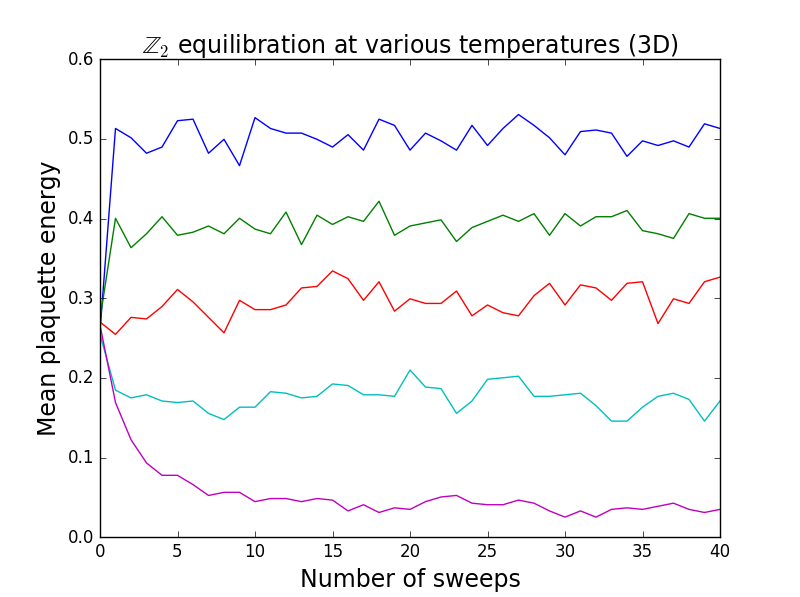
\includegraphics[width=\columnwidth]{equilibration}
	\caption[$\mathbb{Z}_2$ lattice gauge theory phase diagram for a 3D lattice.]{Equilibration of a 3D, $\mathbb{Z}_2$ lattice gauge theory.  From a phase boundary initial condition, the system is equilibrated by sweeping the lattice repeatedly.  The curves shown correspond to inverse temperatures $\beta$ of 0, .4, .8, 1.2, or 1.6, where the higher curves correspond the lower values of $\beta$ (i.e. higher temperatures).  It is seen that it takes only about 5 sweeps at most to reach equilibrium.}
	\label{equilibration}
	\end{centering}
\end{figure}

\section{Results}
I've done simulations for various discrete local symmetry groups: the cyclic groups $\mathbb{Z}_N$ for various values of $N$, the Klein 4-group $K_4$, and the quaternion group Q.  We'll examine each of these cases separately.

\subsection{$\mathbb{Z}_N$}
$\mathbb{Z}_N$ is just the group of integers (mod N), with addition as the group operation.  An isomorphic description is as set of $N^{th}$ roots of unity, with the group operation being multiplication of complex numbers.  This group is Abelian, so each element is in a conjugacy class by itself, and thus any function on the group is a candidate plaquette action.  In addition to the baseline plaquette action, another plaquette action of interest is given by 
\[s(j) = \frac{1}{2}\left(1-\cos\left(\frac{2\pi j}{N}\right)\right) = \frac{1}{2}\left(1 - \Re{\left\{ e^{2\pi i j/N} \right\}}\right),\]
where we are representing group elements by $j=0,1,...,N-1$.  The factor of $\frac{1}{2}$ is chosen to make this action take values in the range $[0,1]$, so that it is more directly comparable to the baseline action (which also takes value in $[0,1]$).  The reason this alternative action is interesting is that, in the limit as $N\rightarrow \infty$, it reduces to the plaquette action for a $U(1)$ lattice gauge theory (as arises in e.g. lattice quantum electrodynamics).  We won't look at $U(1)$, but we will look at this alternative action.  

We start with the simplest case: $\mathbb{Z}_2$ in 2 dimensions.  Note that for $\mathbb{Z}_2$ the baseline action and the alternative action given above are identical, so we will only mention the baseline action.  Sweeping from $\beta=0$ to $\beta=2$ and back (in 80 steps each way) yields the phase diagram (average plaquette energy vs. $\beta$) of fig. (\ref{z2,2d}).
\begin{figure}[h!]
	\begin{centering}
	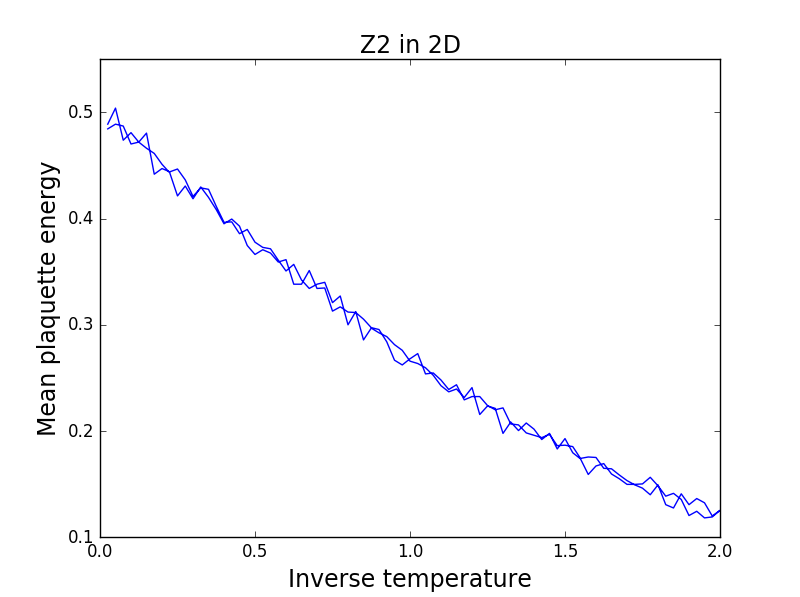
\includegraphics[width=\columnwidth]{z2,2d}
	\caption[$\mathbb{Z}_2$ lattice gauge theory phase diagram for a 2D lattice.]{$\mathbb{Z}_2$ lattice gauge theory phase diagram for a 2D, 15 by 15 lattice.  There are no phase transitions.}
	\label{z2,2d}
	\end{centering}
\end{figure}

This has the expected coarse features---high energy at high temperature (low $\beta$) and low energy at low temperature---but there is no apparent structure, i.e. no apparent phase transition.  This is good, because 2D $\mathbb{Z}_2$ LGT is known analytically to have no phase transition (just a single disordered phase).  Actually, this is the case for all of our gauge groups, so I won't bother to show any more phase diagrams for 2D lattices.  It's good to see one, though, as a sanity check.  

In 3D, we have the phase diagram shown in fig. (\ref{z2,3d}).
\begin{figure}[h!]
	\begin{centering}
	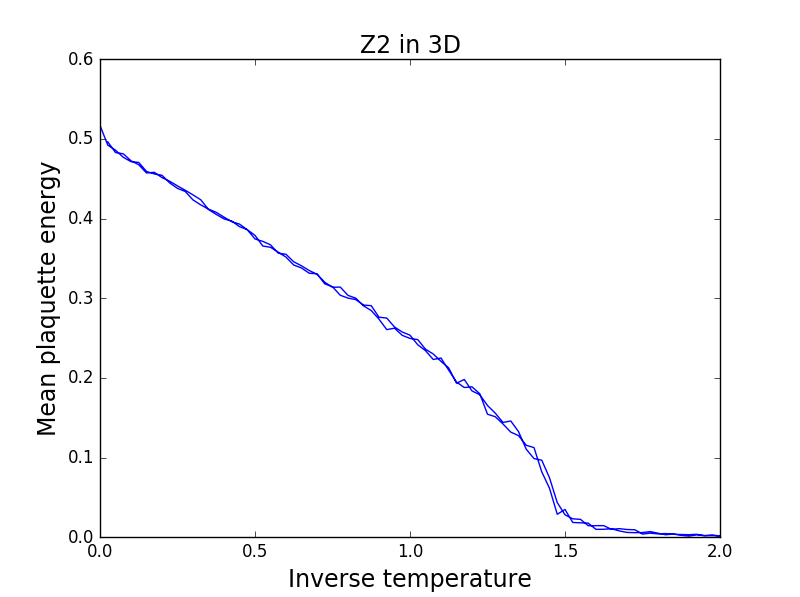
\includegraphics[width=\columnwidth]{z2,3d}
	\caption[$\mathbb{Z}_2$ lattice gauge theory phase diagram for a 3D lattice.]{$\mathbb{Z}_2$ phase diagram for a 3D, 7 by 7 by 7 lattice.  The drop at around $\beta=1.5$ betrays a phase transition there.}
	\label{z2,3d}
	\end{centering}
\end{figure}
This time, we see clear structure---a sharp drop---around $\beta=1.5$, indicating a phase transition.  However, there does not appear to be substantial hysteresis around this phase transition (you'll know what I mean by ``substantial hysteresis'' when you see the higher dimensional LGT phase diagrams).  What we have discovered is that the phase transition of this lattice gauge theory is \textit{continuous}.  This fact is also known analytically: the 3D $\mathbb{Z}_2$ lattice gauge theory is exactly dual to the 3D Ising model, and the since the latter has a continuous phase transition, so must this LGT.

Proceeding to 4D, we now see clearly a hysteresis loop at $\beta \approx .9$, as shown in fig. (\ref{z2,4d}).
\begin{figure}[h!]
	\begin{centering}
	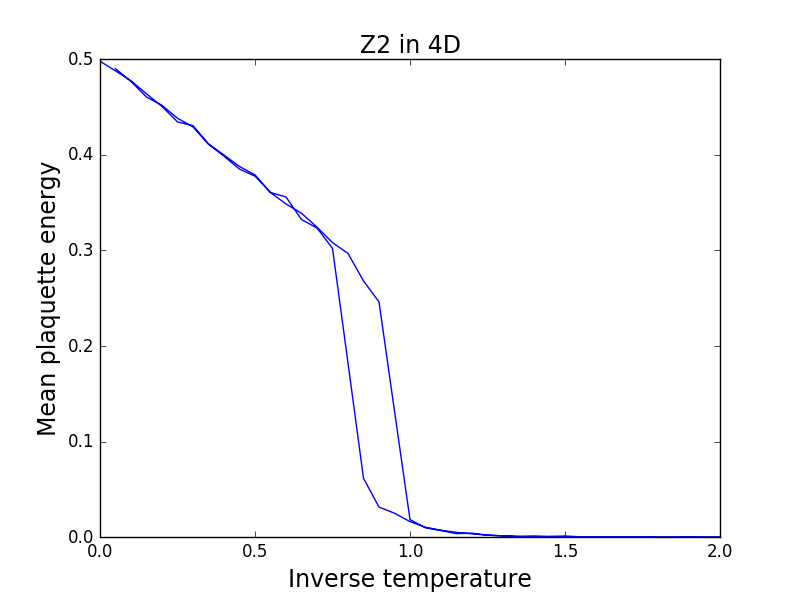
\includegraphics[width=\columnwidth]{z2,4d}
	\caption{$\mathbb{Z}_2$ phase diagram for a 4D, 5 by 5 by 5 by 5 lattice.  The hysteresis loop betrays a phase transition at around 1.4.}
	\label{z2,4d}
	\end{centering}
\end{figure}
We can zero in on this phase transition using the phase boundary method, the results of which are shown in fig. (\ref{z2,4d,phase}).
\begin{figure}[h!]
	\begin{centering}
	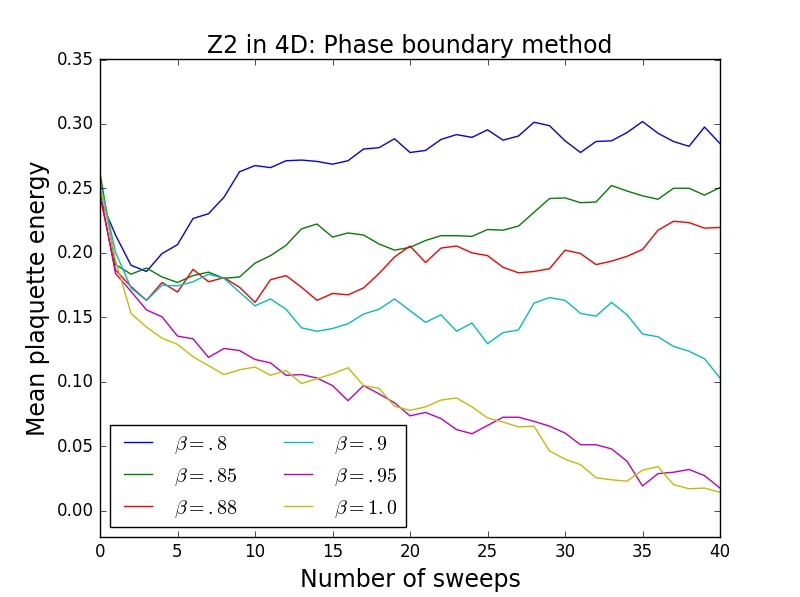
\includegraphics[width=\columnwidth]{z2,4d,phase}
	\caption{The phase transition region for $\mathbb{Z}_2$ LGT on a 4D, 5 by 5 by 5 by 5 lattice, using the phase boundary method.}
	\label{z2,4d,phase}
	\end{centering}
\end{figure}

The phase boundary method pins the critical point at around $\beta= .88$, where the plaquette energy tends neither up nor down at a rapid pace.  In principle, we can attain still better accuracy via this method by looking at more values of $\beta$ and more sweeps (unlike the hysteresis loops, which don't get appreciably more accurate by running more detailed simulations).  However, my own interest undergoes a transition to a deconfined phase beyond about 2 decimal places.  So we'll call it good here. 

For good measure, the phase diagram for $\mathbb{Z}_2$ in 5D is shown in fig. (\ref{z2,56d}).  For \textit{really} good measure, the phase diagram for 6D is also shown.  (I get high on dimensions.)  The hysteresis loops are a little wider, and the transition temperature is a little lower, but they are qualitatively similar to the 4D case. 

\begin{figure}[h!]
	\begin{centering}
	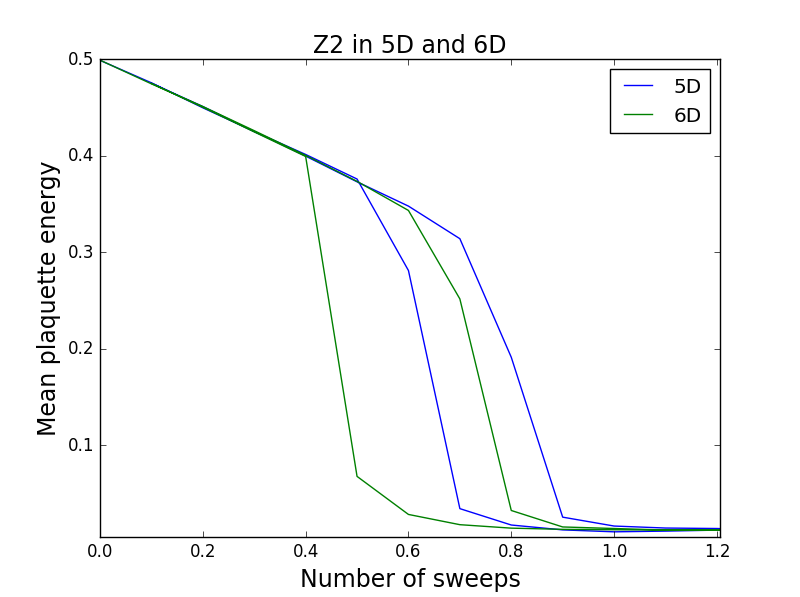
\includegraphics[width=\columnwidth]{z2,56d}
	\caption{$\mathbb{Z}_2$ phase diagram for a 5D, 5 by 5 by 5 by 5 by 5 lattice and for a 6D 5 by 5 by 5 by 4 by 4 by 4 lattice.}
	\label{z2,56d}
	\end{centering}
\end{figure}

I promise I won't do this many dimensions again.  

\begin{figure*}[p]
	\centering
	\subfigure{
		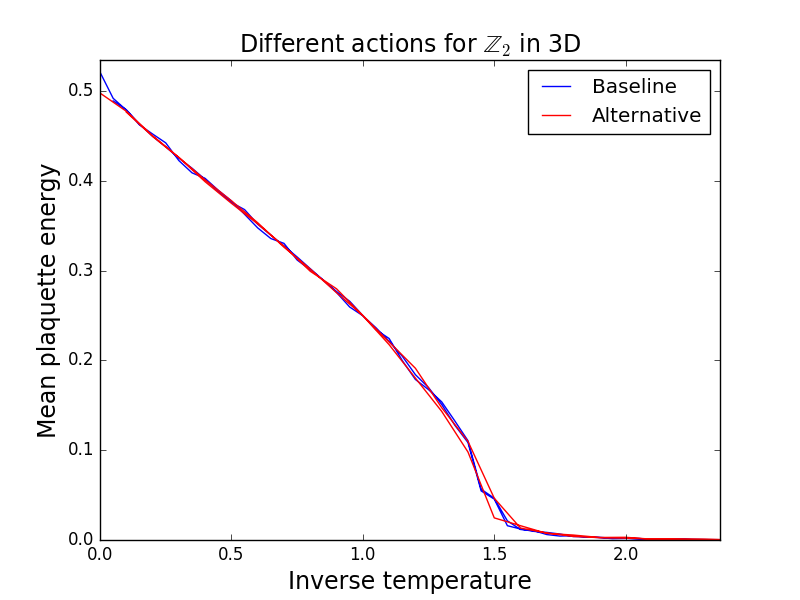
\includegraphics[width=.9\columnwidth]{z2actions,3d}
		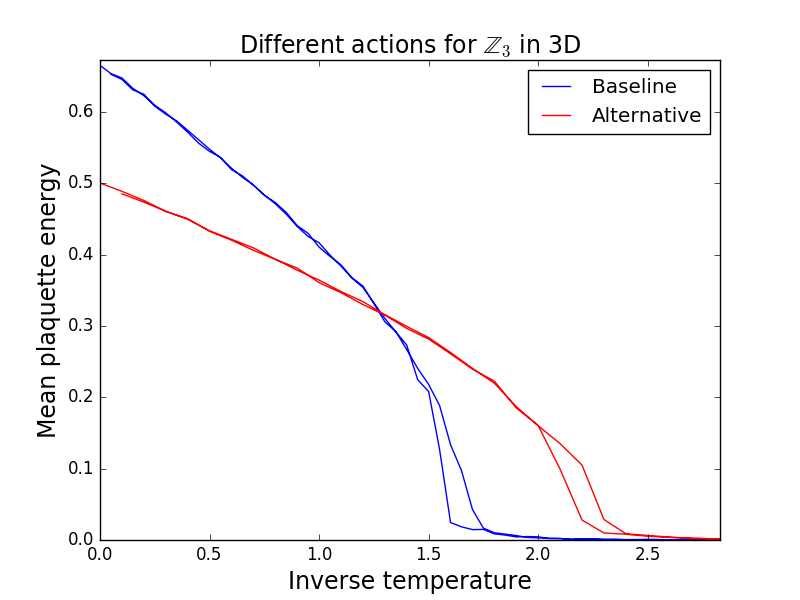
\includegraphics[width=.9\columnwidth]{z3actions,3d}
	}
	\subfigure{
		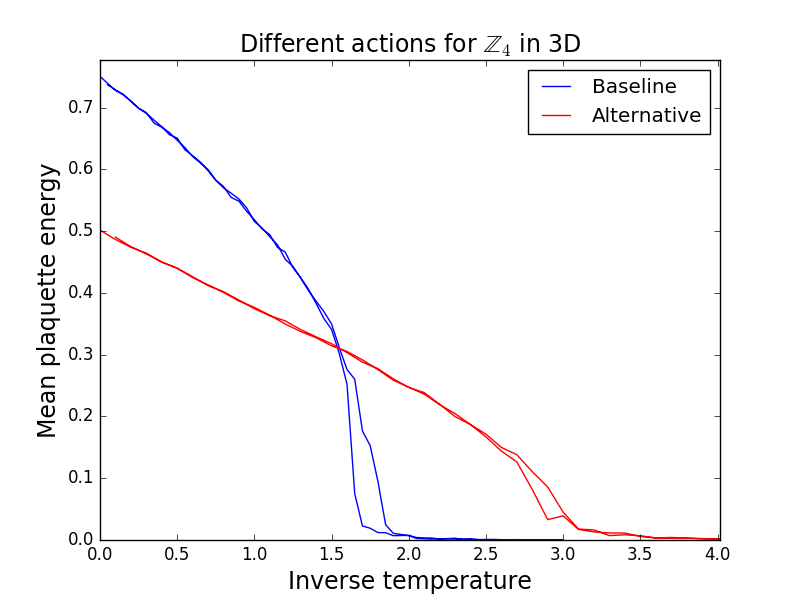
\includegraphics[width=.9\columnwidth]{z4actions,3d}
		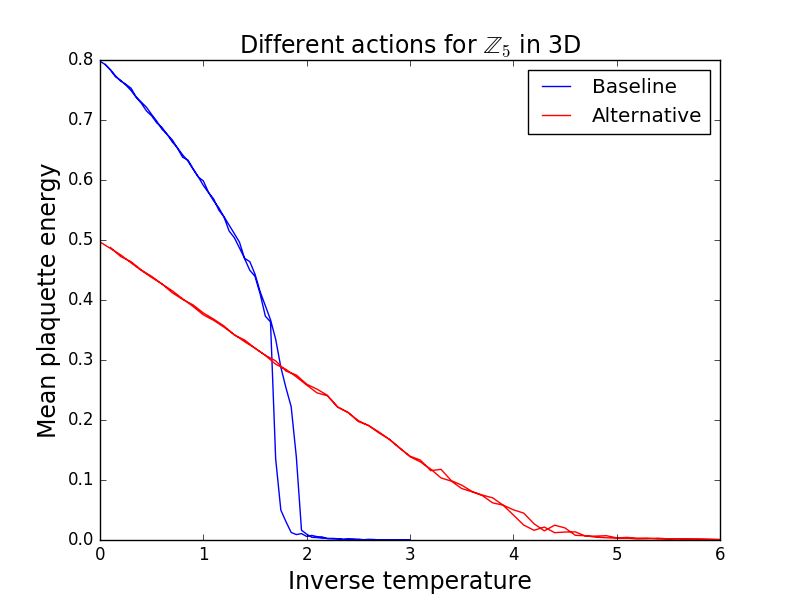
\includegraphics[width=.9\columnwidth]{z5actions,3d}
	}
	\subfigure{
		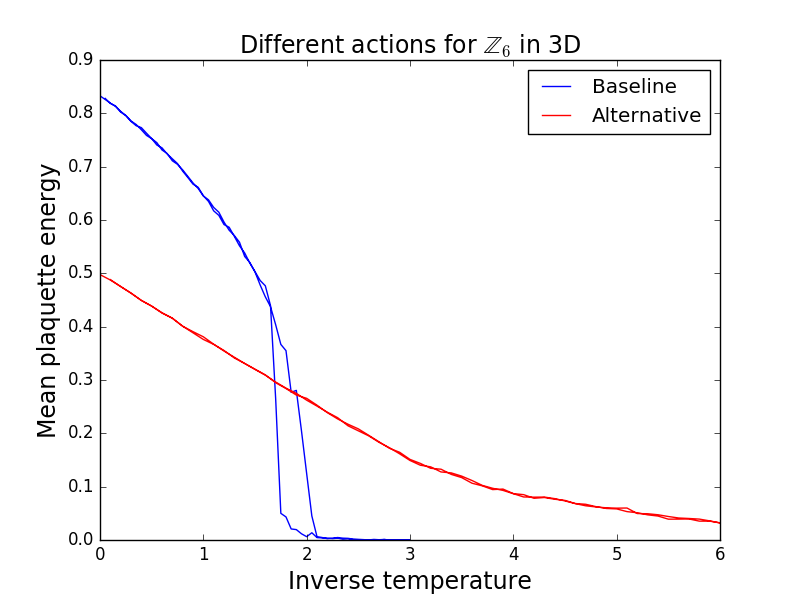
\includegraphics[width=.9\columnwidth]{z6actions,3d}
		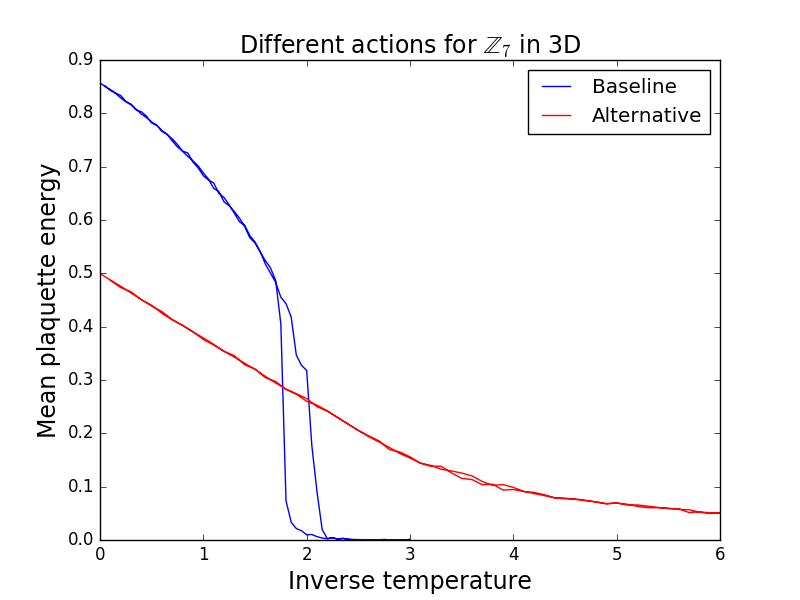
\includegraphics[width=.9\columnwidth]{z7actions,3d}
	}
	\caption{$\mathbb{Z}_N$ phase diagrams for a 3D, 7 by 7 by 7 lattice, for various $N$, and for two different types of action.}
	\label{znactions}
\end{figure*}

\newpage


Having seen all the details in the $\mathbb{Z}_2$ case, I'll expedite the analysis of $\mathbb{Z}_N$ for other values of $N$.  To summarize:  In 3D with the baseline action, $\mathbb{Z}_N$ displays a first order phase transition for all $N>2$.  For the alternative action, for $N\leq4$ we again see a first order phase transition, but with a different critical temperature than for the baseline action.  More interesting is the case of $N\geq 5$, where the alternative action seems to have a higher order phase transition---no sharp hysteresis.  The data I have is too noisy to identify unambiguously the nature of these phase transitions. The comparison between baseline and alternative actions for various $N$ is shown in fig. (\ref{znactions}).  

\begin{figure}[h!]
	\begin{centering}
	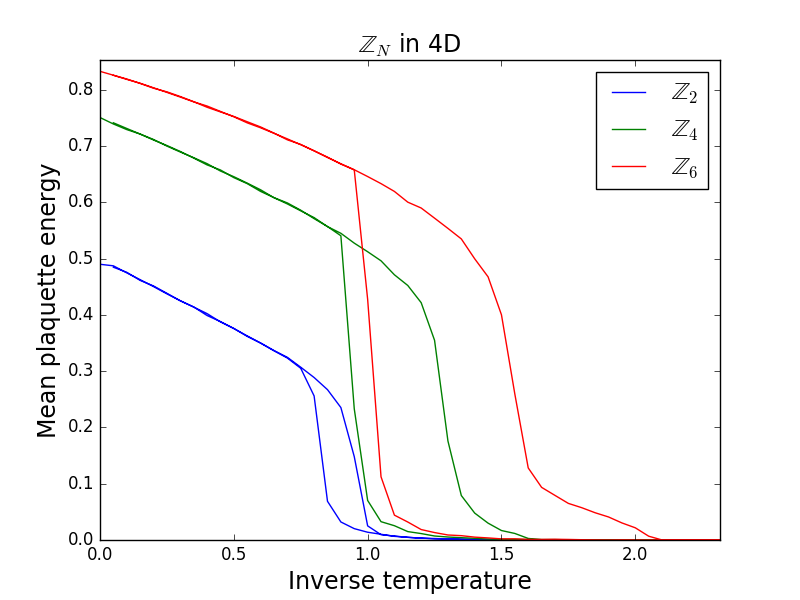
\includegraphics[width=\columnwidth]{zn,4d}
	\caption{$\mathbb{Z}_N$ phase diagrams for a 4D, 7 by 7 by 7 by 7 lattice, for various $N$.}
	\label{zn,4d}
	\end{centering}
\end{figure}

\begin{figure}[h!]
	\begin{centering}
	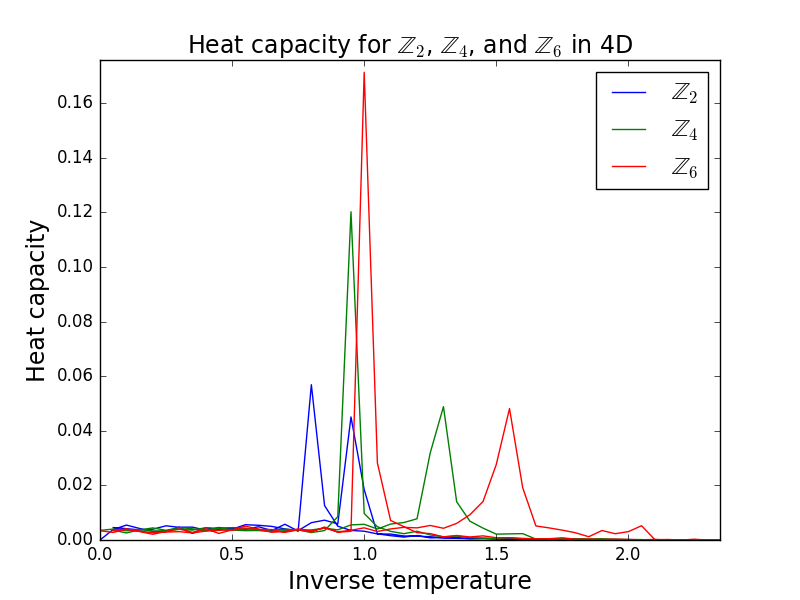
\includegraphics[width=\columnwidth]{heatcapz2z4z6,4d}
	\caption{$\mathbb{Z}_N$ capacities for a 4D, 7 by 7 by 7 by 7 lattice, for various $N$.  Note the blip on the far right for $\mathbb{Z}_6$: this may be a second phase transition. }
	\label{heatcapz}
	\end{centering}
\end{figure}

In 4D, I've only tested the baseline action, the results of which are shown in fig. (\ref{zn,4d}).  The main difference is that $\mathbb{Z}_2$ now clearly displays a first order transition, rather than a continuous transition.  For other values of $N$ the results are qualitatively similar to 3D. 

Something I have not mentioned yet is the heat capacity.  Around a first order phase transition, we expect to see a divergence in the heat capacity.  And indeed, for the 4D $\mathbb{Z}_N$ LGTs we do see divergences in heat capacity around the phase transitions, as shown in fig. (\ref{heatcapz}).

\subsection{Klein 4-group}
The Klein 4-group $K_4$ is interesting primarily because it is the smallest group which is not cyclic, i.e. the smallest group that's not $\mathbb{Z}_N$ for some $N$.  It has 4 elements (as you probably guessed from the name, ``Klein''), which I'll call 1, a, b, and c, and its multiplication table is

\begin{table}[h!]
\centering
Multiplication table for $K_4$

\begin{tabular} {c | c c c c }
& 1 & a & b & c \\
\hline
1 & 1 & a & b & c \\
a & a & 1 & c & b \\
b & b & c & 1 & a \\
c & c & b & a & 1 \\
\end{tabular}
\end{table}

You can verify from this table that $K_4$ is still Abelian, so in some sense it's not \textit{so} different from $Z_4$, the cyclic group with the same number of elements.  And indeed, we find that the phase diagrams for the two groups are virtually identical.  I've plotted them both together in fig. (\ref{k4vz4}) for 3D and 4D.

\begin{figure}[h!]
	\begin{centering}
	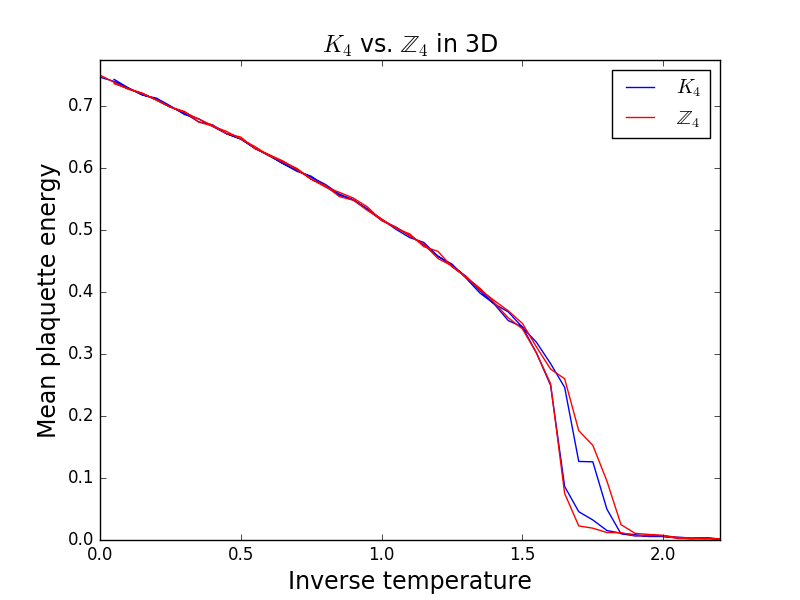
\includegraphics[width=\columnwidth]{k4vz4,3d}
	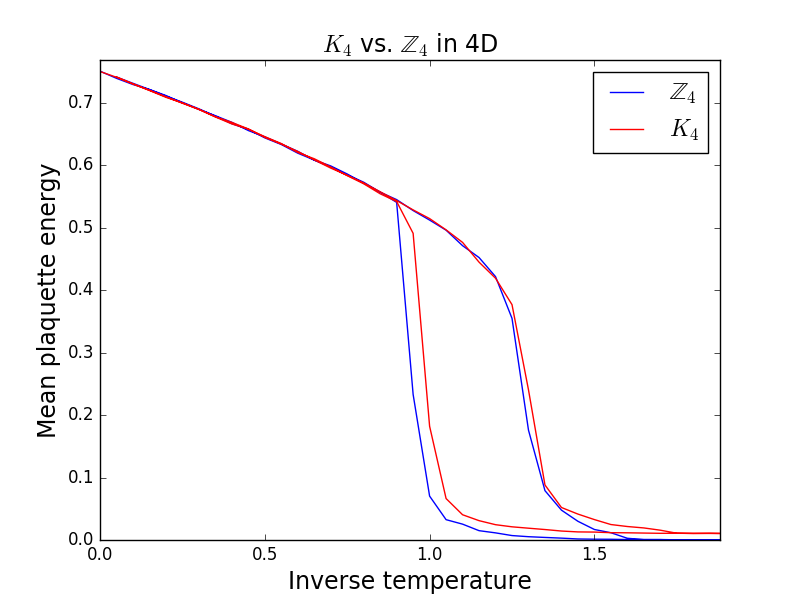
\includegraphics[width=\columnwidth]{k4vz4,4d}
	\caption{Phase diagram of $K_4$, compared against $\mathbb{Z}_4$, for a 3D, 7 by 7 by 7 lattice and for a 4D 7 by 7 by 7 by 7 lattice.}
	\label{k4vz4}
	\end{centering}
\end{figure}

\subsection{Quaternion group}
The quaternion group Q is one of the smallest non-Abelian groups (not quite \textit{the} smallest---that distinction goes to the dihedral group $D_6$).  It has eight elements $\pm1,\pm i, \pm j, \pm k$ and multiplication defined by the rules:
\begin{itemize}
\item $i^2=j^2=k^2=ijk=-1$
\item $\pm1$ commutes with all group elements
\end{itemize}
I'll forgo writing out the full multiplication table.  

The conjugacy classes of Q are $\{1\},\{-1\},\{i,-i\},\{j,-j\},\{k,-k\}$.  The fact that not all group elements are in their own conjugacy classes (a necessary and sufficient condition for non-Abelian-ness) means that there are now some actions for $\mathbb{Z}_8$ (the cyclic group of the same order as Q) which have no analog in Q.  However, for the baseline action (which does offer a meaningful comparison between $\mathbb{Z}_8$ and Q) I find that there is essentially no difference in the phase structure of Q vs. $\mathbb{Z}_8$, just as was found for the comparison of the Klein 4-group vs. $\mathbb{Z}_4$.  The phase diagram of Q and $\mathbb{Z}_8$ in 3D and 4D is shown in fig. (\ref{qvz8}). 

\begin{figure}[h!]
	\begin{centering}
	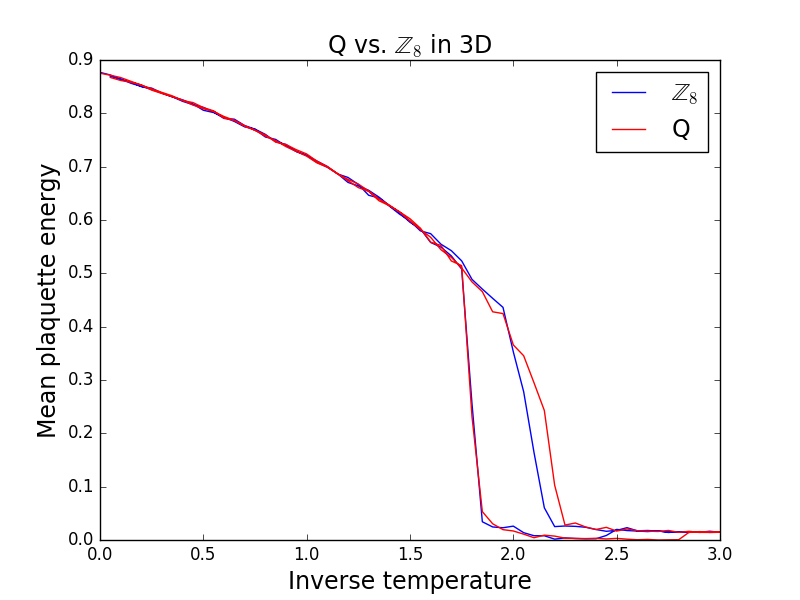
\includegraphics[width=\columnwidth]{qvz8,3d}
	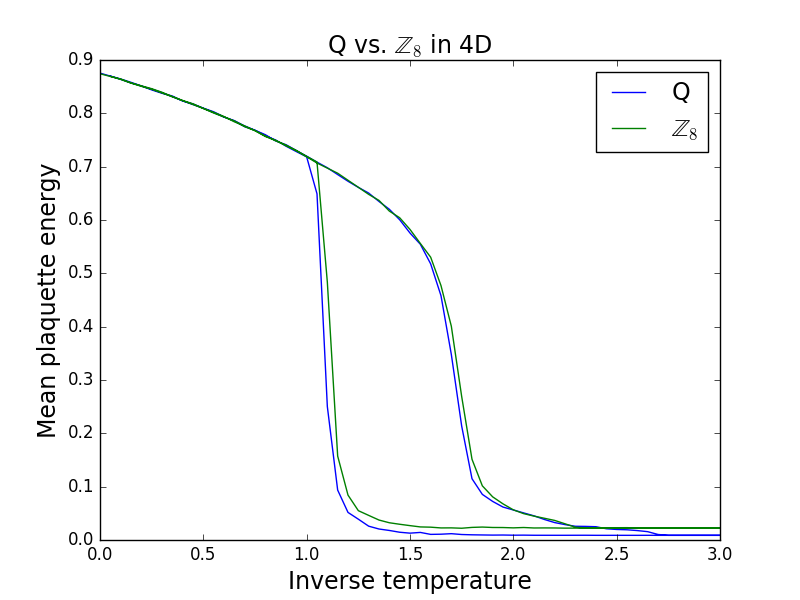
\includegraphics[width=\columnwidth]{qvz8,4d}
	\caption{Phase diagram of Q, compared against $\mathbb{Z}_8$, for a 3D, 7 by 7 by 7 lattice and for a 4D 7 by 7 by 7 by 7 lattice.}
	\label{qvz8}
	\end{centering}
\end{figure}

Because it's kind of pretty, I'll show what a slice of a quaternion LGT looks like at the critical temperature; see fig. (\ref{qcrosssection}).

\begin{figure}[h!]
	\begin{centering}
	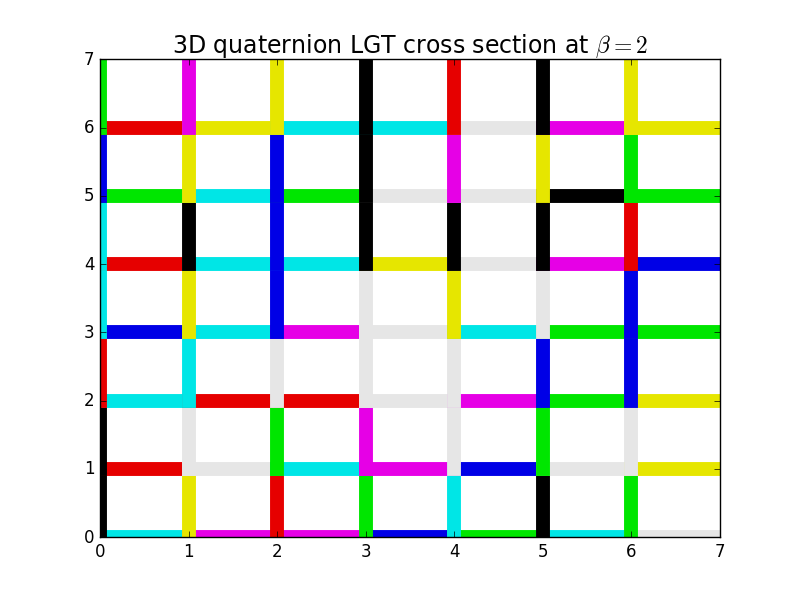
\includegraphics[width=\columnwidth]{qcrosssection}
	\caption{A cross section of a quaternion LFT on a 3D, 7 by 7 by 7 lattice at $\beta=2$.  Different edge colors represent different group elements (black is the identity).}
	\label{qcrosssection}
	\end{centering}
\end{figure}


\section{Conclusions}
I have performed Monte Carlo simulations of various lattice gauge theories to determine their phase structure.  At the most general level, the main conclusion is that the choice of action and lattice dimension and the \textit{order} of the local symmetry group have an important effect on the phase diagram of an LGT, whereas the exact structure of the local symmetry group seems to be less important (insofar as different groups can be compared).  That the choice of local symmetry group is less significant is illustrated by the similarity of the phase diagrams for groups $K_4$ vs. $\mathbb{Z}_4$ and Q vs. $\mathbb{Z}_8$.  Note that this conclusion is not entirely obvious \textit{a priori}, since there are different ways for the product around a plaquette to be the group identity (or any other group element) in, say Q vs. $\mathbb{Z}_8$.  Clearly, though, this has lesser effect than the order of the group on the resulting phase structure.  It would be interesting to consider more non-trivial actions than the baseline action we have been working with, to see if this makes any difference.  (The only reason I have not done so is for lack of time.)

%%%%%%%%%% Bibliography

\begin{thebibliography}{9}

\bibitem{Creutz} 
	M. Creutz, L. Jacobs, and C. Rebbi, 
	Monte Carlo study of Abelian lattice gauge theories, 
	Physical Review D 20.8 (1979): 1915.

\bibitem{Munster}
	G. Münster and M. Walzl,
	Lattice gauge theory-A short primer
	arXiv preprint hep-lat/0012005. 2000 Dec 5.

\bibitem{DAdda}
	A. D’Adda and P. Provero,
	Two-Dimensional Gauge Theories of the Symmetric Group S n in the Large-n Limit
	Communications in mathematical physics 245.1 (2004): 1-25.

\bibitem{Rebbi}
	C. Rebbi,
	Phase structure of non-Abelian lattice gauge theories,
	Physical Review D. 1980 Jun 15;21(12):3350.

\bibitem{Grosse}
	H. Grosse and H. Kühnelt,
	Phase structure of lattice gauge theories for non-abelian subgroups of SU (3)
	Physics Letters B. 1981 Apr 30;101(1):77-81.

\bibitem{Billo}
	M. Billo, A. D'Adda, and P. Provero,
	Branched coverings and interacting matrix strings in two dimensions,
	Nuclear Physics B 616.3 (2001): 495-516.

%\bibitem{BeckRobins} M. Beck and S. Robins, \textit{Computing the Continuous Discretely}, second edition, Springer-Verlag, New York, 2015, \url{http://dx.doi.org/10.1007/978-0-387-46112-0}

\end{thebibliography}

\end{document}